%%%%%%%%%%%%%%%%%%%%%%%%%%%%%%%%%%%%%%%%%%%%%%%%%%%%%%%%%%%%%%%%%%%%%%%%%%%%%
% 26/05/2010
% edited by Bill Lampos
%
% 06.11.2012
% Edited by Magnus Kirø
%
% Feel free to use (copy) the structure (latex formatting source code)
% but not the content of this document.
%
% Latex related packages that you might need: 
%
% texlive-base - TeX Live: Essential programs and files
% texlive-fonts-recommended - TeX Live: Recommended fonts
% latex-xcolor - Easy driver-independent TeX class for color
% texlive-pictures - TeX Live: Graphics packages and programs
% preview-latex-style - extraction of elements from LaTeX documents as graphics
% pgf - TeX Portable Graphic Format
% texlive-binaries - Binaries for TeX Live
% texlive-latex-recommended - TeX Live: LaTeX recommended packages
% texlive-pstricks - TeX Live: PSTricks packages
% texlive-math-extra - TeX Live: Advanced math typesetting
% texlive-latex-base - TeX Live: Basic LaTeX packages
% latex-beamer - LaTeX class to produce presentations
% texlive-latex-extra - TeX Live: LaTeX supplementary packages
% rubber - automated system for building LaTeX documents
% lacheck - Simple syntax checker for LaTeX
% tex-gyre - scalable PostScript and OpenType fonts based on URW Fonts
% texlive-latex-extra-doc - TeX Live: Documentation files for texlive-latex-extra
%
%%%%%%%%%%%%%%%%%%%%%%%%%%%%%%%%%%%%%%%%%%%%%%%%%%%%%%%%%%%%%%%%%%%%%%%%%%%%%
\documentclass[compress,blue]{beamer}
\mode<presentation>

\usetheme{Warsaw}
% other themes: AnnArbor, Antibes, Bergen, Berkeley, Berlin, Boadilla, boxes, CambridgeUS, Copenhagen, Darmstadt, default, Dresden, Frankfurt, Goettingen,
% Hannover, Ilmenau, JuanLesPins, Luebeck, Madrid, Maloe, Marburg, Montpellier, PaloAlto, Pittsburg, Rochester, Singapore, Szeged, classic

%\usecolortheme{whale}
% color themes: albatross, beaver, beetle, crane, default, dolphin, dov, fly, lily, orchid, rose, seagull, seahorse, sidebartab, structure, whale, wolverine

%\usefonttheme{serif}
% font themes: default, professionalfonts, serif, structurebold, structureitalicserif, structuresmallcapsserif

% pdf is displayed in full screen mode automatically
%\hypersetup{pdfpagemode=FullScreen}

% define your own colours:
\definecolor{Red}{rgb}{1,0,0}
\definecolor{Blue}{rgb}{0,0,1}
\definecolor{Green}{rgb}{0,1,0}
\definecolor{magenta}{rgb}{1,0,.6}
\definecolor{lightblue}{rgb}{0,.5,1}
\definecolor{lightpurple}{rgb}{.6,.4,1}
\definecolor{gold}{rgb}{.6,.5,0}
\definecolor{orange}{rgb}{1,0.4,0}
\definecolor{hotpink}{rgb}{1,0,0.5}
\definecolor{newcolor2}{rgb}{.5,.3,.5}
\definecolor{newcolor}{rgb}{0,.3,1}
\definecolor{newcolor3}{rgb}{1,0,.35}
\definecolor{darkgreen1}{rgb}{0, .35, 0}
\definecolor{darkgreen}{rgb}{0, .6, 0}
\definecolor{darkred}{rgb}{.75,0,0}

\xdefinecolor{olive}{cmyk}{0.64,0,0.95,0.4}
\xdefinecolor{purpleish}{cmyk}{0.75,0.75,0,0}

% \usepackage{beamerinnertheme_______}
% inner themes include circles, default, inmargin, rectangles, rounded

%\usepackage{beamerouterthemesmoothbars}
% outer themes include default, infolines, miniframes, shadow, sidebar, smoothbars, smoothtree, split, tree

\useoutertheme[subsection=false]{smoothbars}

% to have the same footer on all slides
%\setbeamertemplate{footline}[text line]{xxx xxx xxx}
%\setbeamertemplate{footline}[text line]{} % or empty footer

% include packages
\usepackage[utf8]{inputenc}
\usepackage[english]{babel}
\usepackage{subfigure}
\usepackage{multicol}
\usepackage{amsmath}
\usepackage{epsfig}
\usepackage{graphicx}
\usepackage[all,knot]{xy}
\xyoption{arc}
\usepackage{url}
\usepackage{multimedia}
\usepackage{hyperref}
\usepackage{setspace}

\title{A Comparison of Approaches to\\ Large-Scale Data Analysis}
\subtitle{}
\author{Magnus Kirø}
\date{\scriptsize Norwegian University of Science and Technology \\ \vspace{.10cm} \today }


% here begins the presentation content. 
\begin{document}

\frame{
	\titlepage
}

\section[Outline]{}
\subsection*{}

%\subsection{Overview}
\frame{\frametitle{Presentation Goals}
The purpose of paper is to consider MapReduce and parallel Database Management Systems for large-scale data analysis. 

\vspace{0.25cm}
\begin{enumerate}
	\item \textbf{Parallel DBMS} and \textbf{MR}, two approaches to large-scale data analysis.  
\vspace{0.25cm}
	\item The \textbf{Architectural Elements} of MR and DBMSs.
\vspace{0.25cm}
	\item \textbf{Benchmarks}, tests and results. 
\vspace{0.25cm}
	\item \textbf{Discussion}, which conclusions can we draw from the tests and their results? 
\end{enumerate}
}

\frame{\tableofcontents}


\section{Two Approaches} % - to large scale data analysis. 
\subsection{Architectural differrences of the two approaches}
\frame{\frametitle{Map Reduce (MR)}

\begin{enumerate}
\item It's simplicity makes MR attractive.

\item Basically: Throw data in a bucket and read it when needed. 

\item Only two Functions:
\begin{enumerate}
		\item \textbf{Map}: 
			Map data into files that are stored in the underlying distributed file system. 
		\item \textbf{Reduce}: 
			Compiles the output data from a mapping function to creata a combined result to the query. 
\end{enumerate} 

\item The map and reduce functions have to be implemented. 
\end{enumerate}
}

\frame{
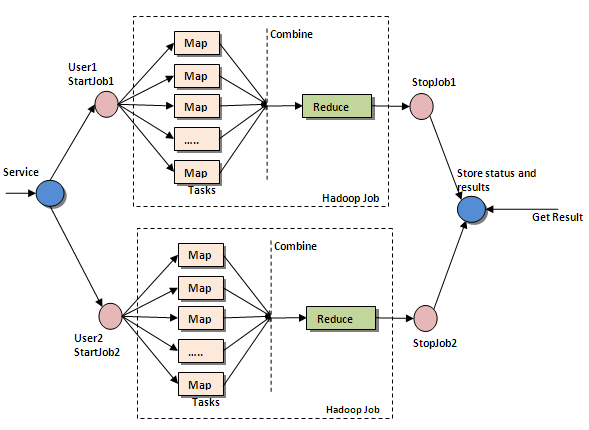
\includegraphics[width=\textwidth]{mapreduce.png}
}

\frame{\frametitle{Parallel Database Management System (DBMS)}
\begin{enumerate}
	\item Tables are partitioned across nodes
	% todo 
	\item Query optimizer, that translates SQL to a query plan. Execution of the query plan is divided among multiple nodes.
	% todo
	\item Underlying storage details can be disregarded by the programmers.
	% todo 
\end{enumerate}
}

\frame{\frametitle{Schema Support}
\begin{enumerate}
\item MR does not have Schema support. Manual data integrity enforcement is required.  
\item DBMS has Schema support. Data integrity is automatically enforced by the schema. 
\end{enumerate}
}

\frame{\frametitle{Indexing}
\begin{enumerate}
\item MR does not have inbuildt indexing. Again the programmer has to implement it, if the functionality is wanted. 
\item DBMS provides indexing. 
\end{enumerate}
}

\frame{\frametitle{Programming Model}
\begin{enumerate}
\item MR, Codasyl style, provide an algorithm to get the data you want.  
\item DBMS, Relational style, state what you want. 
\end{enumerate}
}

\frame{\frametitle{Data Distribution}
\begin{enumerate}
\item MR: get all documents, then compute the result. 
\item DBMS: distributes code to all nodes, the nodes compute partial answers, answers are combined into the result. 
\end{enumerate}
}

\frame{\frametitle{Execution Strategy}
\begin{enumerate}
\item MR: Pull data. Nodes*Maps files - potentially a severe performance problem.  
\item DBMS: Push data.
\end{enumerate}
}

\frame{\frametitle{Flexibility}
\begin{enumerate}
\item MR has the most flexibility. You can do nearly whatevery you want. But you have to enforce your own rules. 
\item DBMS is strict and limited, but comes with great support after a long development time and lots of use. 
\end{enumerate}
}

\frame{\frametitle{Fault Tolerance}
\begin{enumerate}
\item MR: Node crash - task is recheduled to another node. Only that subtask is lost in computing time. 
\item DBMS: Node crash - the whole transaction has to be restarted. Might be very expensive. 
\end{enumerate}
}


\section{Benchmark}
\subsection{The different tasks of the benchmark and it's execution}
\frame{\frametitle{Environment}
\begin{enumerate}
\item Hadoop, DBMS-X and Vertica. 
\item Hadoop whitout compression. The rest with.  
\item Task execution: Each task was executed three times. 
\item All systems was optimized for the tasks given.
\end{enumerate}
}

\frame{\frametitle{Grep Task}
\begin{enumerate}
\item Scan all files for a string pattern.  
\item 100byte records, 10byte key, 90 byte random data. once in every 10.000 records. 
\item Hadoop: Command line to copy data to FS. Significant startup cost. 
\item DBMS: Hash aware load data. 
\item Vertica: Provides a copy cmd. 
\end{enumerate}
}

\frame{
\frametitle{Grep Load Times}
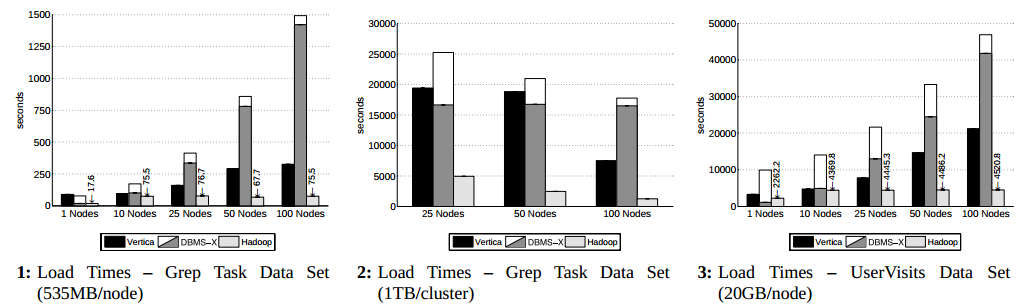
\includegraphics[width=\textwidth]{grep.png}
}

\frame{
\frametitle{Grep Task Results}
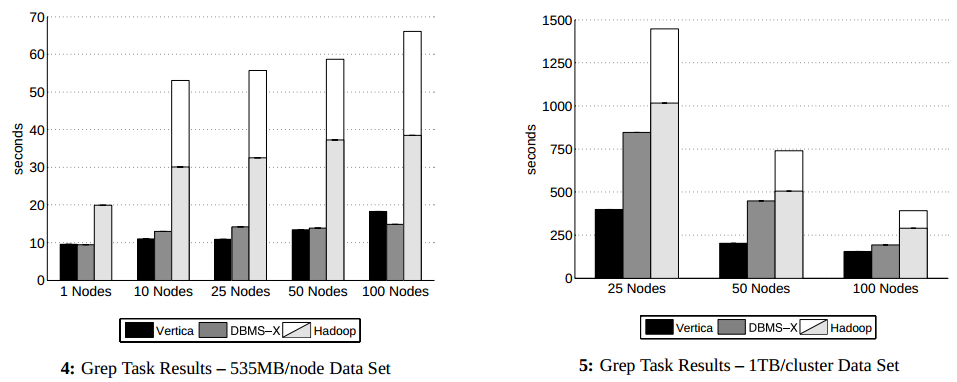
\includegraphics[width=\textwidth]{grepres.png}
}

\frame{\frametitle{Selection Task}
\begin{enumerate}
\item 36.000 data records per file on each node. 
\item Hadoop: Fisnishes so quickly that a torrent of controll messages increases the total execution time. 
\item Again Hadoop is outperformed by the other two. 
 
\end{enumerate}
}

\frame{
\frametitle{Selection Task Results}
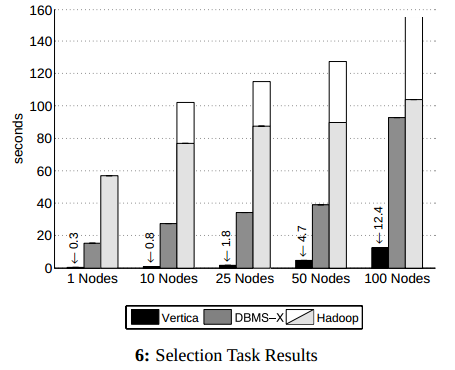
\includegraphics[width=\textwidth]{selection.png}
}

\frame{\frametitle{Aggregation Task}
\begin{enumerate}
\item Task: calculate total revenue by IP. 
\item Produces 2.5 million records(53MB) and 2.000 records(24KB). 
\item Vertica slows down. But does not read unnecessary data columns. 
\item Hadoop: finds all elements of correct type, then sums up the results.  
\end{enumerate}
}

\frame{
\frametitle{Aggregation Task Results}
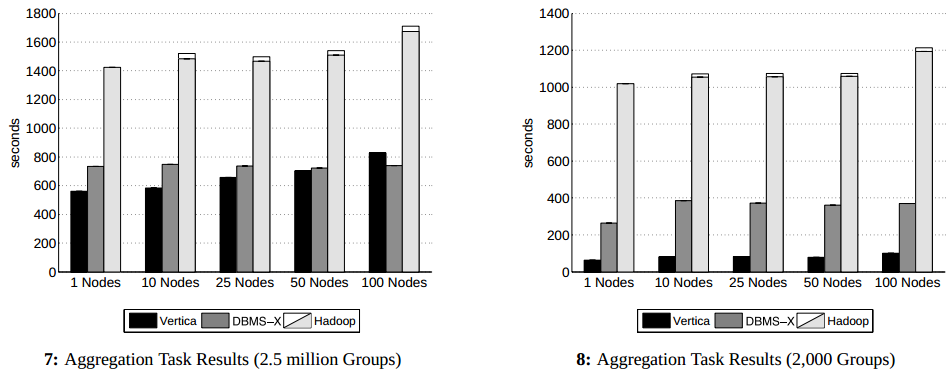
\includegraphics[width=\textwidth]{aggregation.png}
}

\frame{\frametitle{Join Task}
\begin{enumerate}
\item Task: Page rankings in a time period. 
\item Complex MR program with three phases. 
\item Reading and processing data is the most time consuming.  
\end{enumerate}
}

\frame{
\frametitle{Join Task Results}
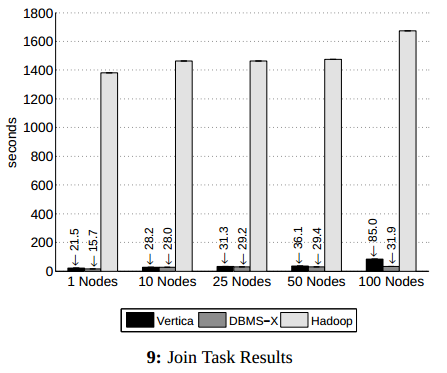
\includegraphics[scale=0.5]{join.png}
}

\frame{\frametitle{UDF Aggregation task}
\begin{enumerate}
\item Task: Counting links in documents.
\item DBMS-X and Hadoop has close to constant execution time. 
\item Result writing gets slower with increased number of nodes.  
\end{enumerate}
}

\frame{
\frametitle{UDF Aggregation Task Results}
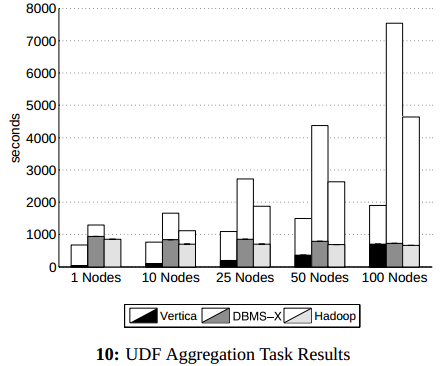
\includegraphics[scale=0.4]{udf.png}
}

\section{Discussion}
\subsection{Pros and cons of the results and setup}
\frame{\frametitle{Install} 
\begin{enumerate}
\item Hadoop: Easy install, trial and error optimization. Task tuning. 
\item DBMS-X: Straight forward install. But the configuration proved difficult. 
\item Vertica: Quite easy install. But too automated tuinig capabilities. 
\end{enumerate}
}

\frame{\frametitle{Task Startup}
\begin{enumerate}
\item MR: 10 sec until the task is distributed. 25 sec for all nodes to start executing. 
\item Hadoop reuse JVM reduced startup time by 10-15\%
\item DBMS: startup time was one of the first things that was improved.
\item Resent improvements (article from 2009). 
\end{enumerate}
}

\frame{\frametitle{Compression}
\begin{enumerate}
\item Both DBMS-X and Vertica worked better with data compression. 
\item Hadoop worked better without compression. 
\end{enumerate}
}

\frame{\frametitle{Data Loading}
\begin{enumerate}
\item Hadoop was the best system to load and read data. 
\item Hadoop was more CPU intensive. 
\item DBMSs can reorganize data on load. 
\end{enumerate}
}

\frame{\frametitle{Exectuion Strategies}
\begin{enumerate}
\item Hadoops overhead messaging slowed it down. 
\item DBMS data push strategy
\item DBMS query plan. 
\end{enumerate}
}

\frame{\frametitle{Failure Models}
\begin{enumerate}
\item More HW = more failures. 
\item MR is more tolerant to failure. 
\item Sophisticated error recovery could improve performance. 
\end{enumerate}
}

\frame{\frametitle{Ease of Use}
\begin{enumerate}
\item MR(Hadoop) was easier to get up and running. Simple structure. But algorithms have to be implemented.  
\item DBMS: might be easier to maintain later. Less data enforecement to do. 
\end{enumerate}
}

\frame{\frametitle{Additional Tools}
\begin{enumerate}
\item DBMS have a long history of development and have a lot of extrernal tools to use. 
\item MR is still young so there is not to many tools available yet. 
\end{enumerate}
}


\section{Conclusion}
\subsection{Summary of solutions and drawbacks}
\frame{\frametitle{Conclusion and Thoughts}
\begin{enumerate}
\item Small scale data analysis will work better with DBMSs. 
\item Large scale data analysis today is way bigger then it was in 2009. 
\item Hadoop and MR systems has room for improvement and will probably be improved over time. 
\item Both architectures will probably remain, due to their different strenghts and areas of use. 
\end{enumerate}
}

\section*{}
\frame{
    \begin{center}
        \huge
        Last slide,\\
        \vspace{1cm}
        Questions?
    \end{center}
}

\end{document} 
